\section*{Question 4}

\paragraph{(a)} We modify equation (7) only. The non-employment income becomes
\[
  \pi_t = \pi_0 + \pi_1 \cdot \mathbf{1}(t \geq 10) \cdot \mathbf{1}(y_t \geq 8), \tag{7$'$}
\]
where $\pi_1 = 0.6$ and $y_t = t + b$. All other equations are unchanged. Because workers have perfect foresight, equation (7$'$) enters the Bellman equation from the first period onward, as workers account for the future subsidy when optimising, even well before becoming eligible.

Note that the year condition $\mathbf{1}(y_t \geq 8)$ is slack: since $y_t = t + b \geq t$, any worker old enough to satisfy $t \geq 10$ automatically has $y_t \geq 10 > 8$. The binding restriction is therefore the age condition $t \geq 10$ alone, and the subsidy is effectively paid to all non-employed workers aged 10 or older. The earliest this can occur is year 10, when cohort $b=0$ first reaches age 10.

\textit{Implementation note:} the PDF uses 1-indexed age ($t \in \{1,\ldots,T\}$) and year, while the code uses 0-indexed variables. To keep the threshold numbers readable and matching the PDF, the conditions are written as \texttt{(t+1) >= 10} and \texttt{(year+1) >= 8} in the code.

\paragraph{(b)}

\begin{figure}[H]
  \centering
  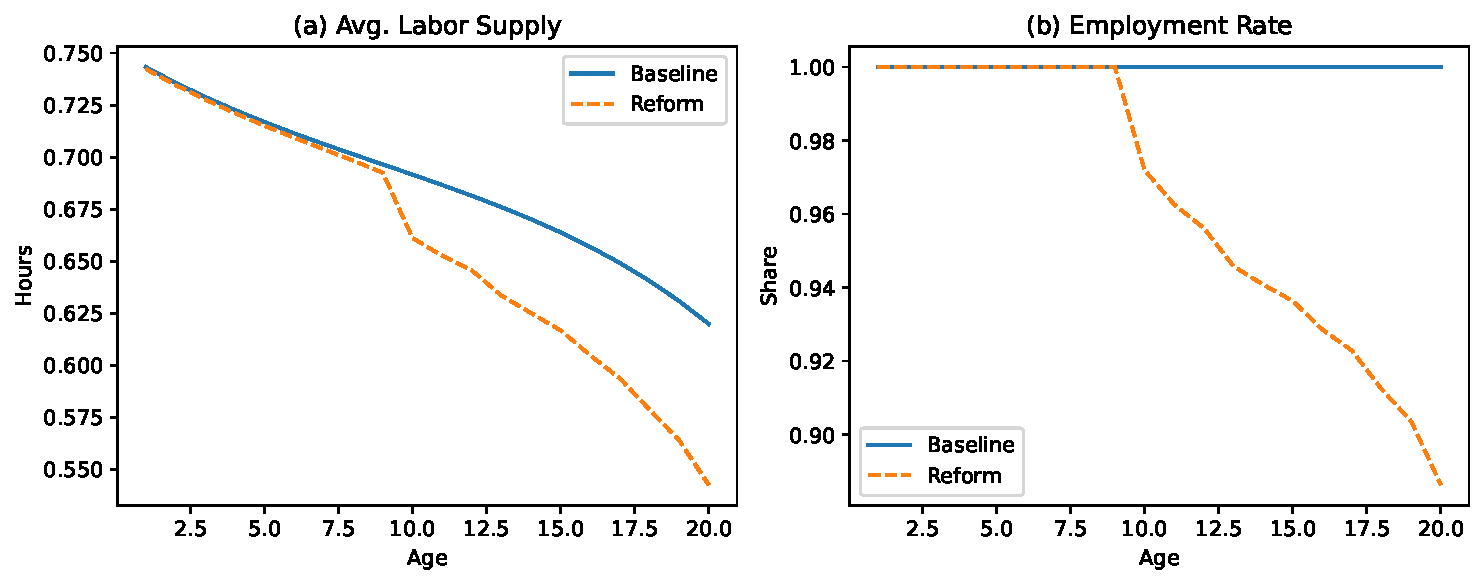
\includegraphics[width=\textwidth]{../figures/q4_age_profiles.pdf}
  \caption{Age profiles for the baseline ($\pi_1 = 0$) and the reform ($\pi_1 = 0.6$).}
  \label{fig:q4_age}
\end{figure}

Average labor supply is nearly identical through age 9, with only a small anticipation effect visible under the reform. From age 10 onward, where the first age at which the $\pi_1$ subsidy applies, we see that labor supply falls as non-employment becomes attractive. The employment rate stays at 100\% in the baseline throughout, but under the reform it begins to drop at age 10 and declines steadily to roughly 89\% by age 20. We thereby see an 11 percentage-point gap driven by workers who prefer the higher $\pi_1$ subsidy over their diminishing after-tax wage late in the life cycle.

\paragraph{(c)}

\begin{figure}[H]
  \centering
  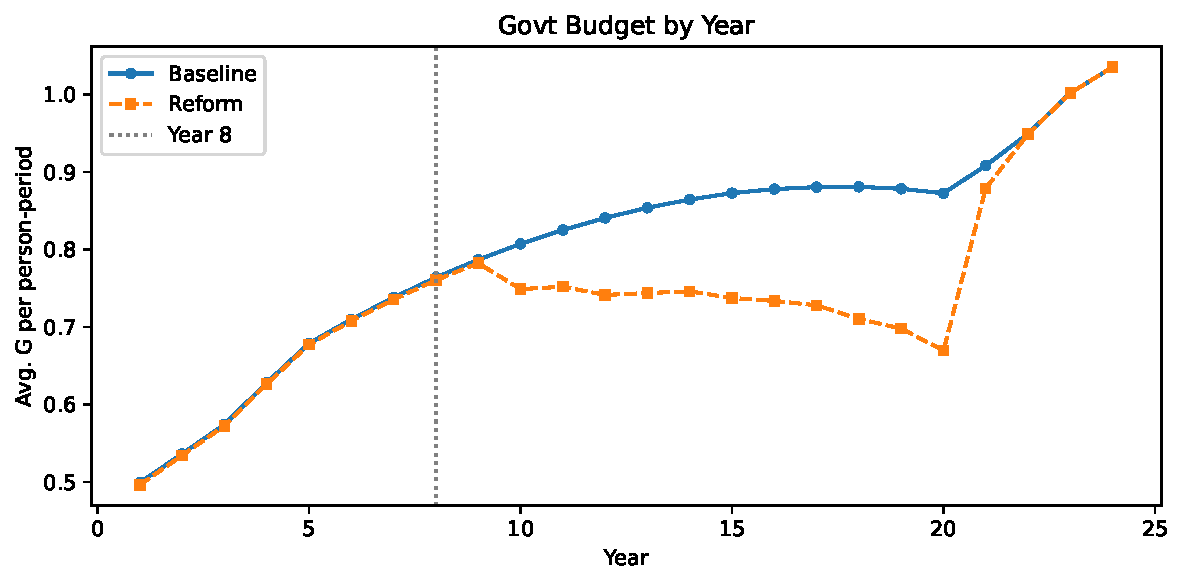
\includegraphics[width=0.7\textwidth]{../figures/q4_govt_by_year.pdf}
  \caption{Average government budget balance per person-period by calendar year.}
  \label{fig:q4_govt}
\end{figure}

The two models are essentially identical through year 9 (only a negligible anticipation wiggle is visible). The reform then diverges sharply downward from year 10 onward, not year 8, because, as noted in part (a), the subsidy cannot be paid until a worker reaches age 10, and the earliest cohort ($b=0$) only reaches that age in year 10. From there the additional subsidy $\pi_1$ raises expenditures for older non-employed workers while reduced employment shrinks the tax base, so net government revenue falls relative to the baseline through the remainder of the simulation.
